\documentclass{book}
\usepackage[utf8]{inputenc}
\usepackage{amssymb}
\usepackage{amsthm}
\usepackage{mathrsfs}
\usepackage{amsmath}  
\usepackage{tkz-euclide}
\usepackage{graphics}  
\usepackage{centernot}
\usepackage{mathtools}
\usepackage{bbding} %五角星
\usepackage{tikz-cd}
\usepackage{hyperref}
\newtheorem{defi}{Definition}[section]
\newtheorem{thm}[defi]{Theorem}
\newtheorem{lem}[defi]{Lemma}
\newtheorem{cor}[defi]{Corollary}
\newtheorem*{remark}{Remark}
\newtheorem{conj}[defi]{Conjecture}
\newtheorem{prop}[defi]{Proposition}
\newtheorem{eg}[defi]{Example}
\newtheorem{q}[defi]{Question}
\newtheorem{try}[defi]{Try to do}
\newtheorem{counter}[defi]{Counterexample}
\numberwithin{equation}{section}
\title{Analysis and Topology}
\author{}
\date{}

\begin{document}

\maketitle
\tableofcontents
\chapter{Limit}
\section{L'Hopital's Rule}
Some examples that can not apply L'Hopital's rule.
\begin{eg}
$$
 \lim_{x\to +\infty} \frac{1}{x}\int_0^x|\sin(t)|dt.
$$
\end{eg}
\begin{proof}
    This is because 
    $$
    \lim_{x\to \infty} \frac{f^\prime (x)}{g^\prime (x)}
    $$ does not exist. One can use squeeze theorem to show that the limit is $2/\pi.$
\end{proof}

\begin{eg}
$$
 \lim_{x\to +\infty} \frac{x}{\sqrt{x^2+1}}.
$$
\end{eg}
\begin{proof}
    When using L'hopital's rule, one will get
 $$
 \lim_{x\to +\infty} \frac{\sqrt{x^2+1}}{x}. 
$$  And doing it again, it goes back to
$$
 \lim_{x\to +\infty} \frac{x}{\sqrt{x^2+1}}.
$$  We can just divide $x,$ and find the limit is $1.$  
\end{proof}

\begin{eg}
$$
 \lim_{x\to +\infty} \frac{x}{x+\sin(x)}.
$$ 
\end{eg}

\begin{eg}
    $$
 \lim_{x\to 0} \frac{\exp(-1/x^2)}{x^2}.
$$
\end{eg}


\chapter{Differentiation and Integration}
Leibniz integral rule:
$$
\frac{d}{dx}\int_{a(x)}^{b(x)}f(x,t) dt=f(x,b(x))\cdot b^\prime(x)-f(a(x),x)\cdot a^\prime(x)+\frac{d}{dx}\int_{a(x)}^{b(x)}\frac{\partial}{\partial x}f(x,t) dt.
$$

\begin{thm}[The dominated convergence theorem] 
Suppose $f_n: \mathbb{R} \rightarrow [-\infty, \infty]$ are
(Lebesgue) measurable functions such that the pointwise limit $f(x) = \lim_{n\rightarrow \infty}f_n(x)$ exists. Assume there is an integrable $g: \mathbb{R} \rightarrow [0,\infty]$ with $|f_n(x)| \leq g(x)$ for each $x\in\mathbb{R}$. Then $f$ is integrable as is $f_n$ for each $n$, and
$$
\lim_{n\rightarrow \infty} \int_{\mathbb{R}}f_n d\mu=\int_{\mathbb{R}}\lim_{n\rightarrow\infty}f_n d\mu =
\int_{\mathbb{R}}f d\mu.
$$
\end{thm}

\textbf{Applications of the dominated convergence theorem}
\begin{thm}[Continuity of integrals]
Assume $f: \mathbb{R}\times \mathbb{R}\rightarrow \mathbb{R}$ is such that $x\mapsto f(x,t)$ 
is measurable for each $t\in\mathbb{R}$ and $t \mapsto f(x, t)$ is continuous for each $x \in\mathbb{R}$. Assume also that there is an integrable $g : \mathbb{R}\rightarrow \mathbb{R}$ with $|f(x, t)| \leq g(x)$ for each $x, t \in\mathbb{R}$. Then the function
$f(\cdot, t)$ is integrable for each $t$ and the function $F: \mathbb{R} \rightarrow \mathbb{R}$ defined by
$$
F(t) = \int_{\mathbb{R}}f(x,t) d\mu
$$
is continuous.
\end{thm}

\textbf{Fact:} Risch (1969): An algorithm to determine whether the indefinite integral of elementary functions is elementary or not. 


\chapter{Techniques of Integration}
(2023/04/02)\medskip

\textbf{Technique I: Introducing variables (go to higher dimension)}
\begin{eg}
    Calculate 
    $$
     \int_0^\infty \frac{e^{-x}-e^{-2x}}{x} dx.
    $$
\end{eg}
\begin{proof}[(sol.)]
    It is easier to compute if we take it as an integration on $\mathbb{R}^2.$ That is,
    $$
    \int_0^\infty \frac{e^{-x}-e^{-2x}}{x} dx =\int_0^\infty \int_1^2 e^{-yx} dydx = \int_1^2 \int_0^\infty  e^{-yx} dydx=\log(2).
    $$
\end{proof}

\textbf{Note:} One can also use technique III below by considering
\[
I(t)=\int_0^\infty \frac{e^{-tx}-e^{-2x}}{x} dx.
\]

(2023/04/09)\medskip

\textbf{Technique II:Ramanujan's master theorem}

Reference: \href{http://arminstraub.com/downloads/pub/rmt.pdf}{Ramanujan's Master Theorem}
\begin{thm}\label{MasterThm}
    If a complex-value function $f(x)$ has an expansion of the form
    $$
    f(x)=\sum_{k=0}^\infty \frac{\phi(k)(-x)^k}{k!}
    $$ then the Mellin transform of $f(x)$ is given by
    $$
        \int_0^\infty x^{s-1}f(x)dx=\phi(-s)\Gamma(s).
    $$
\end{thm}

Note: Higher-dimensional versions of this theorem also appear in quantum physics (through Feynman diagrams).\medskip

Employing the forward-shift operator $E$ defined by
$E\cdot \lambda(n)=\lambda(n+1).$

\begin{proof}[(Formal proof of \ref{MasterThm})]
This uses some strange integration on operators to get the result.
    \[
        \begin{aligned}
            \int_0^\infty x^{s-1}\sum_0^\infty \frac{(-1)^n}{n!}\lambda(n) x^ndx&=\int_0^\infty x^{s-1}\sum_0^\infty \frac{(-1)^n}{n!}E^nx^n x^ndx\cdot \lambda(0) \\
            &=\int_0^\infty x^{s-1}e^{-Ex}dx\cdot \lambda(0) \\ 
            &=\int_0^\infty \frac{\Gamma(s)}{E^s}\lambda(0)\\
            &=\Gamma(s)\lambda(-s).
        \end{aligned}
    \]
\end{proof}

The rigorous proof of Ramanujan’s Master Theorem provided by Hardy in \cite{H}.
\begin{eg}
    $$
    \int_0^\infty \sin(x^n) dx=\frac{1}{n}\Gamma(\frac{1}{n})\sin(\frac{\pi}{2n}), \; \int_0^\infty \cos(x^n) dx
    $$
\end{eg}
\begin{proof}
    First use change of variable $t=x^n.$
\end{proof}

\textbf{Technique III:Feynman technique (introduce one more variable)}
\begin{eg}
    Calculate
    \[
\int_0^1\frac{x^7-1}{\ln x} dx.
    \]
\end{eg}    
\begin{proof}[(sol.)]
    Let 
    \[
    I(t)=\int_0^1\frac{x^t-1}{\ln x}dx.
    \] Then
    \[
    I^\prime(t)=\frac{d}{dt}\int_0^1\frac{x^t-1}{\ln x}dx=\int_0^1\frac{\partial}{\partial t}\frac{x^t-1}{\ln x}dx=\int_0^1 x^t dx=\frac{1}{t+1}.
    \] Therefore, one has $I(t)=\ln(t+1)+C.$ Since we have $I(0)=0,$ $I(t)=\ln(t+1)$. So the integral equals $\ln 8.$ 
\end{proof}

\textbf{Note:} This problem can also be solved by technique I by using change of variable $y=\ln x$ first. 

\textbf{Technique IV: Contour integration:}
This is a method from complex analysis.
\begin{eg}
\[
\int_0^{2\pi} R(\cos\theta,\sin\theta) d\theta.
\] where $R$ is a rational function.
\end{eg}
\begin{proof}
    One has
    \[
    \cos\theta=\frac{z+z^{-1}}{2}, \; \sin\theta=\frac{z-z^{-1}}{2i}
    \] where $z=e^{i\theta}.$ Thus the integral can be transformed in the form of some rational function of $z$ integrated on the unit circle; hence, one can apply Cauchy residue theorem when the function behave well on the unit circle.
\end{proof}

\chapter{Parametric Equations and Polar Coordinates}
Reference: \cite[Chapter 10]{S}.
\section{Curves Defined by Parametric Equations}
$$
C: x=f(t), \; y=g(t) \; [\textbf{parametric equations}] \quad
$$ where $\alpha\leq t\leq \beta$ [$t$ is called \textbf{parameter}]. \medskip

More general, one can define \textbf{parametrized curves} in $\mathbb{R}^n.$
\begin{eg}
 \textbf{The Cycloid}
 $$
 \begin{aligned}
 x&=r(\theta-\sin{\theta}) \\
  y&=r(1-\cos{\theta})
 \end{aligned}
 $$
 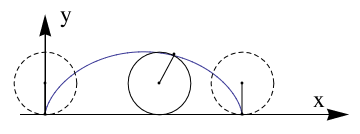
\includegraphics[scale=0.6]{cycloid.png} \medskip
 
 Cycloid is the solution of \textbf{brachistochrone problem} and \textbf{tautochrone problem}.
\end{eg}

\begin{q}
Given a parametrized curve $C$ with parametric equations $x=f(t), y=g(t),$ how can one derive $h(x,y)\in \mathbb{R}[x,y]$ such that $h(f(t),g(t))=0?$ Ask the same question in $\mathbb{R}^n.$
\end{q}

\begin{q}
Conversely, given $h(x,y)\in \mathbb{R}[x,y]$, how can one derive a parametrized curve $C$ with parametric equations $x=f(t), y=g(t)$ such that $h(f(t),g(t))=0 ?$ Ask the same question in $\mathbb{R}^n.$
\end{q}



\chapter{Iterated Limit}

\begin{thm} Let $X$ be a metric space and $f(x,y)$ be a function on $X$.
If $\lim\limits_{x\rightarrow a, y\rightarrow b}f(x,y), \lim\limits_{x\rightarrow a}f(x,y), \lim\limits_{y\rightarrow b}f(x,y)$ exist except at $x=a,y=b.$ $(a,b$ can be $\infty)$ Then
$$
\lim\limits_{x\rightarrow a, y\rightarrow b}f(x,y)=\lim\limits_{y\rightarrow b}\lim\limits_{x\rightarrow a}f(x,y)=\lim\limits_{x\rightarrow a}\lim\limits_{y\rightarrow b}f(x,y).
$$
\end{thm}
\begin{proof}
Since $\lim\limits_{x\rightarrow a, y\rightarrow b}f(x,y)=L$ exists;  therefore, for any $\epsilon >0$ there exists some $\delta$ such that 
$$
|f(x,y)-L|<\epsilon \quad \text{if} \ 0<|x-a|<\delta, \ 0<|y-b|<\delta.
$$ Then
$$
\lim_{x\rightarrow a}|f(x,y)-L|=|\lim_{x\rightarrow a}f(x,y)-L|\leq \epsilon \quad 0<|y-b|<\delta
$$ So,
$$
\lim\limits_{y\rightarrow b}\lim\limits_{x\rightarrow a}f(x,y)=L.
$$ Similarly, we have
$$
\lim\limits_{x\rightarrow a}\lim\limits_{y\rightarrow b}f(x,y)=L.
$$
\end{proof}

\begin{cor}
If $\lim\limits_{i\rightarrow \infty, j\rightarrow \infty}a_{ij}, \lim\limits_{i\rightarrow \infty}a_{ij}, \lim\limits_{j\rightarrow \infty}a_{ij}$ exist, then
$$
\lim\limits_{i\rightarrow \infty, j\rightarrow \infty}a_{ij}=\lim_{j \rightarrow \infty} \lim_{i \rightarrow \infty} a_{ij}=\lim_{i \rightarrow \infty} \lim_{j \rightarrow \infty} a_{ij}.
$$
\end{cor}

\begin{remark}
The condition of the existence of $\lim\limits_{i\rightarrow \infty}a_{ij}, \lim\limits_{j\rightarrow \infty}a_{ij}$ is needed. Since the existence of $\lim\limits_{i\rightarrow \infty, j\rightarrow \infty}a_{ij}$ does not imply the existence of the other two limit. For example, consider $\{a_{ij}\}$ which is defined by \medskip

\begin{tikzpicture}
\matrix(m)[matrix of math nodes,column sep=1cm,row sep=1cm]{
    \vdots & \vdots & \vdots & \vdots \\
    1 & 0 & \frac{1}{3} & 0 & \cdots \\
    0 & \frac{1}{2} & 0 & \frac{1}{3} & \cdots \\
    1 & 0 & \frac{1}{2} & 0 & \cdots \\
    0 & 1 & 0 & 1 &\cdots \\
};
\end{tikzpicture} \medskip

with vertical coordinate $i$, and horizontal coordinate $j.$
\end{remark}

\begin{thm}
Suppose $\lim\limits_{x\rightarrow a}f(x,y), \lim\limits_{y\rightarrow b}f(x,y)$ exist except at $x=a,y=b.$ Then $f(x,y)\rightarrow \lim\limits_{x\rightarrow a}f(x,y)$ locally uniformly at $b$ or $f(x,y)\rightarrow \lim\limits_{y\rightarrow b}f(x,y)$ locally uniformly at $a.$ if and only if $\lim\limits_{x\rightarrow a, y\rightarrow b}f(x,y)$ exists. Therefore if $f(x,y)\rightarrow \lim\limits_{x\rightarrow a}f(x,y)$ locally uniformly at $b$ or $f(x,y)\rightarrow \lim\limits_{y\rightarrow b}f(x,y)$ locally uniformly at $a$ then 
$$
\lim\limits_{y\rightarrow b}\lim\limits_{x\rightarrow a}f(x,y)=\lim\limits_{x\rightarrow a}\lim\limits_{y\rightarrow b}f(x,y).
$$
\end{thm}
\begin{proof}
W.L.O.G., suppose $f(x,y)\rightarrow \lim\limits_{x\rightarrow a}f(x,y)$ locally uniformly at $b.$ Then there exists $\delta >0$ such that $f(x,y)\rightarrow \lim\limits_{x\rightarrow a}f(x,y)$ uniformly on $0<|y-b|<\delta.$ First, we claim that
$\lim\limits_{y\rightarrow b}\lim\limits_{x\rightarrow a}f(x,y)$ exists. Put
$$
l_a(y):=\lim\limits_{x\rightarrow a}f(x,y).
$$ Then for $y,y^\prime$ are closed enough to $b$ and proper $x,$
$$
\begin{aligned}
|l_a(y)-l_a(y^\prime)|& \leq |l_a(y)-f(x,y)|+|f(x,y)-\lim_{y\rightarrow b}f(x,y)|+|\lim_{y\rightarrow b}f(x,y)-f(x,y^\prime)|+|f(x,y^\prime)-l_a(y^\prime)|\\
&< \epsilon.
\end{aligned}
$$ since we can pick $x$ first such that $|l_a(y)-f(x,y)|$ and $|f(x,y^\prime)-l_a(y^\prime)|$ are small then pick $y$ such that the other terms small. Then by Cauchy criterion, the limit exists and we denote it by $L.$ We have 
$$
|f(x,y)-L|\leq |f(x,y)-l_a(y)|+|l_a(y)-L|
$$ if we first pick $y$ closed to $b$, then let $x$ be closed to $a.$ So this means
$$
\lim\limits_{x\rightarrow a, y\rightarrow b}f(x,y)
$$ exists and equal $L.$ \medskip

Conversely, if 
$$
\lim\limits_{x\rightarrow a, y\rightarrow b}f(x,y)
$$ exists and equal $L.$ Then for any $\epsilon >0$, there exists $\delta$ such that
$$
|f(x,y)-L|<\epsilon
$$ if $0<|x-a|<\delta, 0<|y-b|<\delta.$ So
$$
|l_a(y)-f(x,y)|\leq |l_a(y)-L|+|L-f(x,y)|<2\epsilon
$$ if we also let $\delta$ be picked such that $|l_a(y)-L|<\epsilon.$ These means
$$
f(x,y)\rightarrow l_a(y) \ \text{locally uniformly at } b.
$$
\end{proof}

\begin{eg}
 $$
\lim\limits_{y\rightarrow b}\lim\limits_{x\rightarrow a}f(x,y)=\lim\limits_{x\rightarrow a}\lim\limits_{y\rightarrow b}f(x,y)
$$ does not imply $\lim\limits_{x\rightarrow a, y\rightarrow b}f(x,y)
$ exists. For example,
$$
f(x,y)=\left\{
\begin{aligned}
&\frac{xy}{x^2+y^2}, & (x,y)\neq (0,0) \\
&0, & (x,y)=(0,0).
\end{aligned}
\right.
$$
\end{eg}

\begin{q}
Can we find some different properties $\{P_i\}$ such that
$$
\lim\limits_{y\rightarrow b}\lim\limits_{x\rightarrow a}f(x,y)=\lim\limits_{x\rightarrow a}\lim\limits_{y\rightarrow b}f(x,y) \Leftrightarrow P_i.
$$
\end{q}

%%%%%%%%%%%%%%%%%%%%%%%%%%%%%%%%%%%%%%
\section{Interchange of integral}
%%%%%%%%%%%%%%%%%%%%%%%%%%%%%%%%%%%%%%%
\begin{thm}
Let $f(z,t):D \times I \rightarrow \mathbb{C}$ be a continuous function where $I$ is an interval of $\mathbb{R}$ and $D$ is a domain in $\mathbb{C}$. Let $\gamma$ be a smooth curve on complex plane and 
$$
\int_{\gamma}\int_I |f(z,t)|dt dz
$$ converges, then
$$
\int_{\gamma}\int_I f(z,t)dt dz=\int_I \int_{\gamma} f(z,t) dz dt.
$$
\end{thm}
\begin{proof}
First, suppose $I=[a,b]$ Define
$$
F(z):=\int_{a}^b f(z,t)dt, \ F_n(z):=\frac{b-a}{n}\sum_{k=1}^n f(z,a+k(b-a)/n).
$$
By definition of Riemann integral, $F_n(z)\rightarrow F(z)$ as $n$ tends to $\infty$ for any $z.$ Now we claim that the convergence is uniform. Indeed, since we have
$$
\begin{aligned}
|F_n(z)-F(z)|&=\bigg|\sum_{k=1}^n \int_{a+\frac{(k-1)(b-a)}{n}}^{a+\frac{k(b-a)}{n}}[f(z,a+k(b-a)/n)-f(z,t)]dt\bigg| \\
&\leq \sum_{k=1}^n \int_{a+\frac{(k-1)(b-a)}{n}}^{a+\frac{k(b-a)}{n}}\bigg|f(z,a+k(b-a)/n)-f(z,t)\bigg|dt
\end{aligned}
$$ Since continuous function is uniformly continuous on compact set, for large $n$, we have 
$$
\bigg|f(z,a+k(b-a)/n)-f(z,t)\bigg|< \epsilon.
$$
So
$$
|F_n(z)-F(z)|< (b-a)\epsilon.
$$ Therefore, the convergence is uniform. So 
$$
\int_{\gamma}\int_I f(z,t)dt dz=\int_{\gamma} \lim_n F_n(z) dz= \lim_n \int_{\gamma} F_n(z) dz =\int_I \int_{\gamma} f(z,t) dz dt.
$$\medskip

For general $I$, we find $I_n\rightarrow I$ such that $I_n$ is a finite union of $[a_i,b_i].$ Define
$$
G(z):=\int_I f(z,t)dt, \ G_n(z):=\int_{I_n} f(z,t)dt
$$. Again, we can prove that $G_n$ converges to $G$ uniformly since
$$
\int_{\gamma}\int_I |f(z,t)|dt dz
$$ converges; in particular, $\int_I |f(z,t)|dt$ is defined. To be continued...
\end{proof}

%%%%%%%%%%%%%%%%%%%%%%%%%%%%%%%%
\section{Infinite product}
%%%%%%%%%%%%%%%%%%%%%%%%%%%%%%%%%%
\begin{defi}
Let $\{u_i\}_{i=1}^\infty$ be a sequence of nonzero complex numbers. If $P_N=u_1\cdots u_N$ converges to a nonzero number as $N \rightarrow \infty$, then we say $\prod_{i=0}^\infty u_i$ converges. If $P_N$ converges to $0$, we say the infinite product diverges to $0.$ If only finitely many $u_i$ are zero, and $\prod_{u_i \neq 0}^\infty u_i$ converges, then we say $\prod_i u_i$ converges to zero.
\end{defi}

\begin{prop}
$(1)$ If $\prod u_i$ converges, then $u_i \rightarrow 1.$ So we often write the product as $\prod{(1+z_i)}$ where $z_i$ converges to $0.$\medskip

$(2)$ If ${a_i}$ is a positive real number, then $\prod (1+a_i)$ converges if and only if $\sum a_i$ converges.\medskip

$(3)$ Let $a_i$ be a sequence in $\mathbb{C}\backslash \{-1\}.$ If $\sum_{i=1}^\infty |a_i|^2 <\infty,$ then $\sum_{i=1}^\infty a_i$ and $\prod_{i=1}^\infty (1+a_i)$ converge or diverge together.
\end{prop}
\begin{proof}
(1) Since $u_i= P_i/ P_{i-1},$ letting $i \rightarrow \infty$, $u_i \rightarrow 1.$ \medskip

(2) It follows from 
$$
a_1+\cdots +a_N \leq \prod_i (1+a_i) \leq e^{a_1+\cdots +a_N},
$$ since $1+x\leq e^x.$\medskip

(3)
\end{proof}

\begin{prop}
Let $z_k \neq -1.$ Then $\prod (1+z_k)$ converges if and only if $\sum \log(1+z_k)$ converges. ($\log z$ here denotes the principle branch of the logarithm; i.e $-\pi < \Im \log z= \mathrm{Arg}z \leq \pi.$)
\end{prop}
\begin{proof}
Let $S_N=\sum_{k=1}^N \log (1+z_k).$ Then $P_N=e^{S_N}$. So if $S_N \rightarrow S,$ then $P_N \rightarrow P=e^S.$ Conversely, suppose that $P_N \rightarrow P\neq 0.$ Then, some branch of the log (denote by $\log^*$) is continuous at $P$ and $\log^* P_n \rightarrow \log^* P$ as $N \rightarrow \infty.$ Suppose we inductively define integers $n_k$ by
$$
\sum_{k=1}^N (\log (1+z_k)+2\pi i n_k)=\log^* (P_N).
$$ Then, since $\log^* (P_N)$ converges,
$$
\sum_{k=1}^N (\log (1+z_k)+2\pi i n_k)
$$ converges; therefore $\log (1+z_k)+2\pi i n_k \rightarrow 0$. Since $z_k$ converges to $0$ and $\log$ denotes the principal branch, it follow that $n_k=0$ for $k$ large. Hence $\sum \log(1+z_k)$ converges.
\end{proof}

\begin{prop}
If $\sum_{k=1}^\infty |z_k|$ converges, then $\prod_{k=1}^\infty (1+z_k)$ converges.
\end{prop}
\begin{proof}
It follows from
$$
|\log(1+z_k)|\leq |z_k|(1+\frac{1}{2}+\frac{1}{4}+\cdots)=2|z_k|.
$$
\end{proof}

\begin{defi}
$\prod_{k=1}^\infty (1+z_k)$ is called absolutely convergent if 
$$
\prod_{k=1}^\infty (1+|z_k|) 
$$ converges.
\end{defi}

\begin{prop}
An absolutely convergent product is convergent.
\end{prop}
\begin{proof}
Since the convergence of $\sum |z_k|$ is equivalent to the convergence of $\prod{(1+|z_k|)}.$
\end{proof}

We wish to consider analytic functions defined by infinite products;i.e.,functions of the form 
$$
f(z)=\prod_{k=1}^\infty (1+u_k(z)).
$$

\begin{thm}
Suppose that $u_k(z)$ is analytic in a region $D$ for $k=1,2,\cdots$ and that $\sum_{k=1}^\infty |u_k(z)|$ converges uniformly on compacta. Then the product
$$
\prod_{k=1}^\infty (1+u_k(z)) 
$$ converges uniformly on compacta and represents an analytic function in $D.$
\end{thm}
\begin{proof}
Let $A$ be a compact subset of $D.$ Since $\sum_{k=1}^\infty |u_k(z)|$ converges uniformly on $A,$ for $k$ large, $|u_k(z)|<1$ there. Hence, we can assume $1+u_k \neq 0$ for all $k.$ If we then take $N$ large enough so that $\sum_{k=N+1}^\infty |u_k| <\epsilon/2.$ Then
$$
|\sum_{k=N+1}^\infty \log(1+u_k(z))|\leq \epsilon. 
$$ So $\sum_{k=1}^\infty \log(1+u_k(z))$ converges unif. on $A.$  Finally, since the exponential function is uniformly continuous in any bounded domain,
$$
P_N(z)=\exp \big(\sum_{k=1}^N \log(1+u_k(z))\big)
$$ converges unif.
\end{proof}

\textbf{The Weierstrass Product Theorem}
According to the Uniqueness Theorem, a nontrivial entire function cannot have an accumulation point of zeroes. That is, if $\{\lambda_k\} \rightarrow \lambda$ and if $f$ is an entire function with zeroes at all the points $\lambda_k$, then $f=0$. On the other hand,an entire function may be zero at all the points of a sequence which diverges to $\infty.$

\begin{thm}[Weierstrass]
Suppose $\lambda_k \rightarrow \infty.$ Then there exists an entire function $f$ such that $f(z)=0$ if and only if $z=\lambda_k,$ for $k=1,2,\cdots$
\end{thm}

\textbf{Note:}
 To define an entire function with zeroes at the points $\lambda_k$,it would seem natural to write
 $$
 f(z)=\prod_{k=1}^\infty (z-\lambda_k).
 $$ However, since $\lambda_k \rightarrow \infty,$ the terms of the product would not approach $1$ (for fixed $z$) and hence the product would diverge. Instead, we consider the infinite product of linear functions given by 
 $$
 f(z)=\prod_{k=1}^\infty (1-\frac{z}{\lambda_k}),
 $$ assuming for now that $\lambda_k \neq 0$. Indeed, if $\sum_{k=1}^\infty |\frac{1}{\lambda_k}|$ converges,	$\sum_{k=1}^\infty |\frac{z}{\lambda_k}|$ converges uniformly on every compact set so that the product is uniformly convergent on compacta and gives the desired entire function. If $\sum_{k=1}^\infty |\frac{1}{\lambda_k}|$ diverges, $\sum_{k=1}^\infty |\frac{1}{\lambda_k^2}|$ converges, we consider
 $$
 f(z)=\prod_{k=1}^\infty \bigg[(1-\frac{z}{\lambda_k})e^{z/\lambda_k}\bigg].
 $$ For $|\lambda_k|>2|z|,$
 $$
 \bigg| \log\bigg[(1-\frac{z}{\lambda_k})e^{z/\lambda_k}\bigg]\bigg| \leq |z/\lambda_k|^2. 
 $$ Hence the series
$$
\sum_{k=1}^\infty \log\bigg[(1-\frac{z}{\lambda_k})e^{z/\lambda_k}\bigg], z\neq \lambda_k
$$ is is uniformly convergent and the product is uniformly convergent on compacta. By the same reasoning, if $\sum_{k=1}^\infty |\frac{1}{\lambda_k^{m+1}}|$ converges for some positive integer $m$ and we consider the convergence factors
$$
E_k(z)=\exp{\bigg(z/\lambda_k+z^2/2\lambda_k^2+\cdots + z^m/m\lambda_k^m\bigg)},
$$ it follows that the infinite product 
$$
\prod_{k=1}^\infty (1-\frac{z}{\lambda_k})E_k(z)
$$ is uniformly convergent on compacta and represents an entire function with the desired zeroes. However, there exists some $\{\lambda_k\}$ such that $\lambda \rightarrow \infty$ and $\sum_{k=1}^\infty |\frac{1}{\lambda_k^{N}}|$ diverges for all $N$ (e.g $\{\log k\}$), so for general case we need some modification.


\begin{proof}
Assume for a moment $\lambda_k \neq 0$ and set
$$
E_k(z)=\exp\bigg(\frac{z}{\lambda_k}+\frac{z^2}{2\lambda_k}+\cdots +\frac{z^k}{k\lambda_k^k}\bigg).
$$ Suppose $|z|<M.$ Since $\lambda_k \rightarrow \infty,$ for large $k$, we have $|\lambda_k|>2|z|$ and
$$
\bigg|\log\bigg[(1-\frac{z}{\lambda_k})E_k(z)\bigg]\bigg|\leq \sum_{j=k+1}^\infty \bigg| \frac{z^j}{j\lambda_k^j}\bigg|\leq \bigg|\frac{z}{\lambda_k}\bigg|^k \leq \frac{1}{2^k}.
$$ Hence, both
$$
\sum_{k=1}^\infty \log\bigg[(1-\frac{z}{\lambda_k})E_k(z)\bigg], \ \prod_{k=1}^\infty (1-\frac{z}{\lambda_k})E_k(z)
$$ are uniformly convergent on compacta. Note also that the individual factors are zero only at the points $\lambda_k$,and by the definition of convergence the infinite product is zero at those points only. Finally, if we seek an entire function with zeroes at the origin as well, we need only set
$$
f(z)=z^p \prod_{k=1}^\infty (1-\frac{z}{\lambda_k})E_k(z).
$$
\end{proof}

\begin{eg}
To find an entire function $f$ with a single zero at every negative integer $\lambda_k=-k$, note that $\sum_{k=1}^\infty 1/k^2$ converges, we can take
$$
f(z)=\prod_{k=1}^\infty (1+\frac{z}{k})e^{-z/k}.
$$
\end{eg}

\begin{eg}
 An entire function with a single zero at every integer is given by
$$
f(z)=z\prod_{k=1}^\infty (1-\frac{z}{k})e^{z/k}(1+\frac{z}{k})e^{-z/k}=z\prod_{k=1}^\infty (1-\frac{z^2}{k^2}).
$$
\end{eg}
\begin{prop}
Let
$$
f(z)=z\prod_{k=1}^\infty (1-\frac{z^2}{k^2}).
$$ Then $f(z)=\sin(\pi z)/\pi.$
\end{prop}
\begin{proof}
Skip.
\end{proof}

\section{Riemann zeta function}
Riemann zeta function is defined by
$$
\zeta(s):=\sum_{n=1}^\infty \frac{1}{n^s}
$$ where $\mathrm{Re}(s)>1.$

\begin{prop}
$$
\zeta(s)=\prod_{p}(1-p^{-s})^{-1}.
$$
\end{prop}
\begin{proof}
Define 
$$
f_n(s)=(1-2^{-s})(1-3^{-1})\cdots (1-p_n^{-1})\zeta(s)=1+\sum_{2,3,\cdots,p_n \nmid n} \frac{1}{n^s}.
$$ Since
$$
\sum_{2,3,\cdots,p_n \nmid n} \frac{1}{n^s} \rightarrow 0
$$ as $n\rightarrow \infty,$ we have

$$
\zeta(s)\prod_p (1-p^{-s})^{-1}=1
$$
Also, we know $\prod_p (1-p^{-s})$ converges since it consists of  some of the factors of the absolutely convergent product $\prod_{n=2}^\infty (1-n^{-s})$, so 
$$
\zeta(s)=\prod_{p}(1-p^{-s})^{-1}.
$$
\end{proof}

\chapter{Ordinary Differential Equations}
\begin{defi}
For an ordinary differential equation
$$
y^{(n)}+f_1(x)y^{(n-1)}+\cdots+f_{n-1}(x)y^{\prime}+f_n(x)=Q(x),
$$ we say $x_0 \in \mathbb{R}$ is ordinary if 
$f_1(x), \cdots, f_n(x), Q(x)$ are analytic at $x_0;$ otherwise, we call it a singular point. 
\end{defi}
\chapter{Taylor's formula}
There is a connection between one dimensional Taylor's formula and higher dimensional Taylor's formula.\medskip

Now I just sketch the idea which I still do not have time and mood to write it down: \medskip

$$
e^{x^2+y^2}=1+(x^2+y^2)+\frac{1}{2!}(x^2+y^2)^2+\cdots
$$

\chapter{Measure Theory}
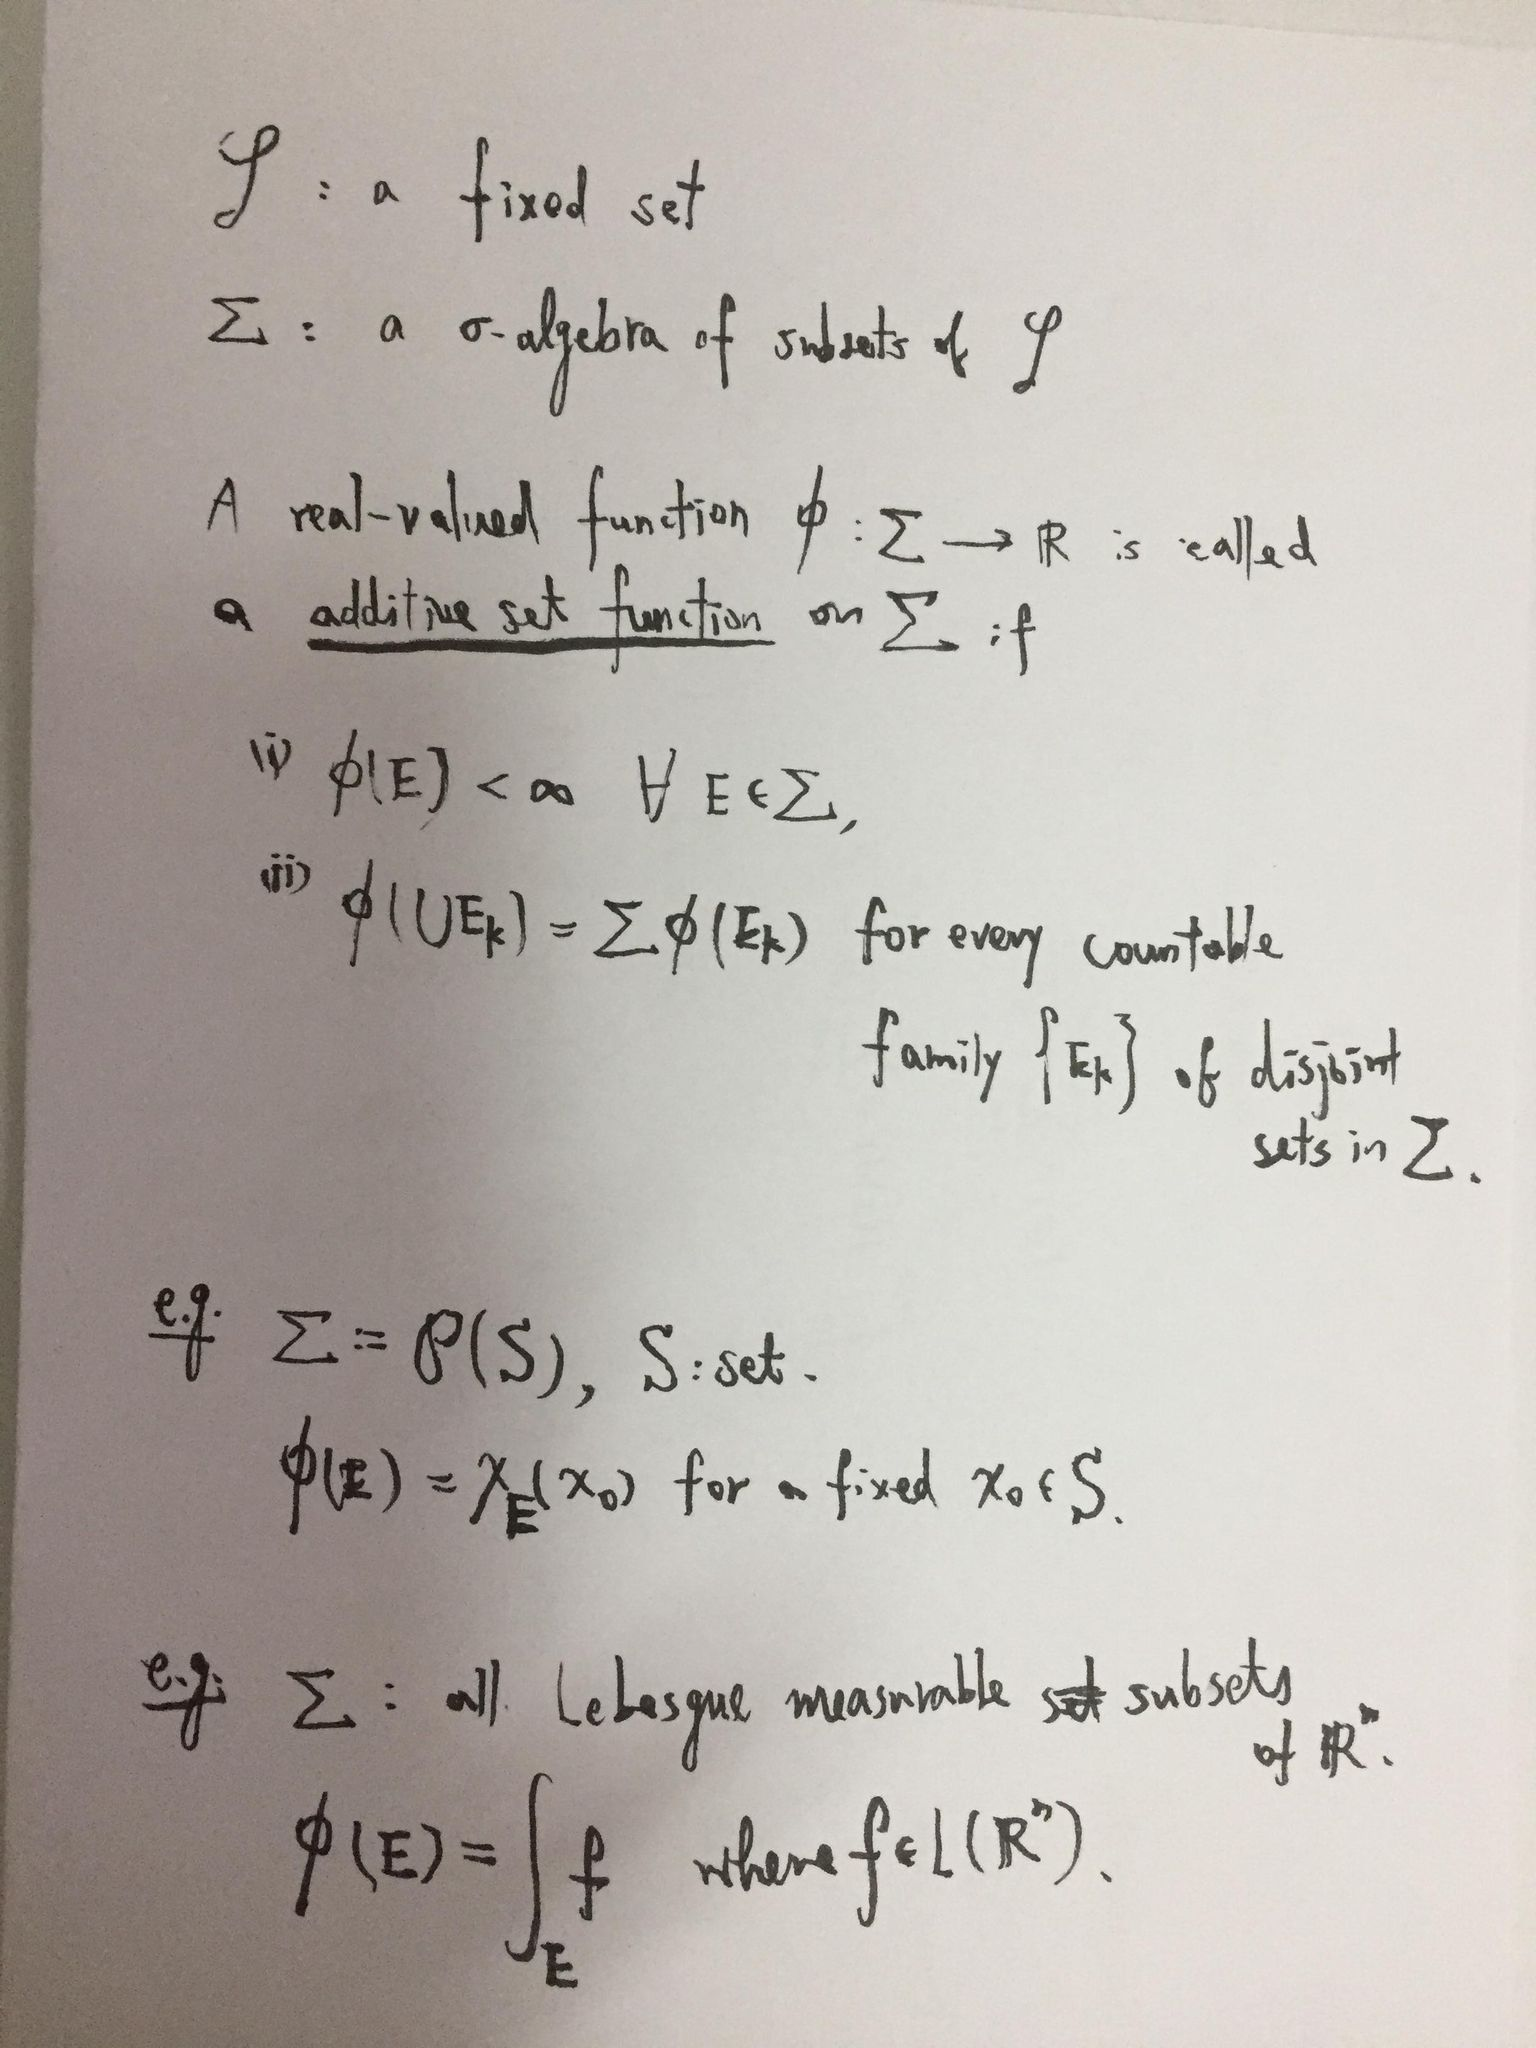
\includegraphics[scale=0.1]{measure_1.jpg} 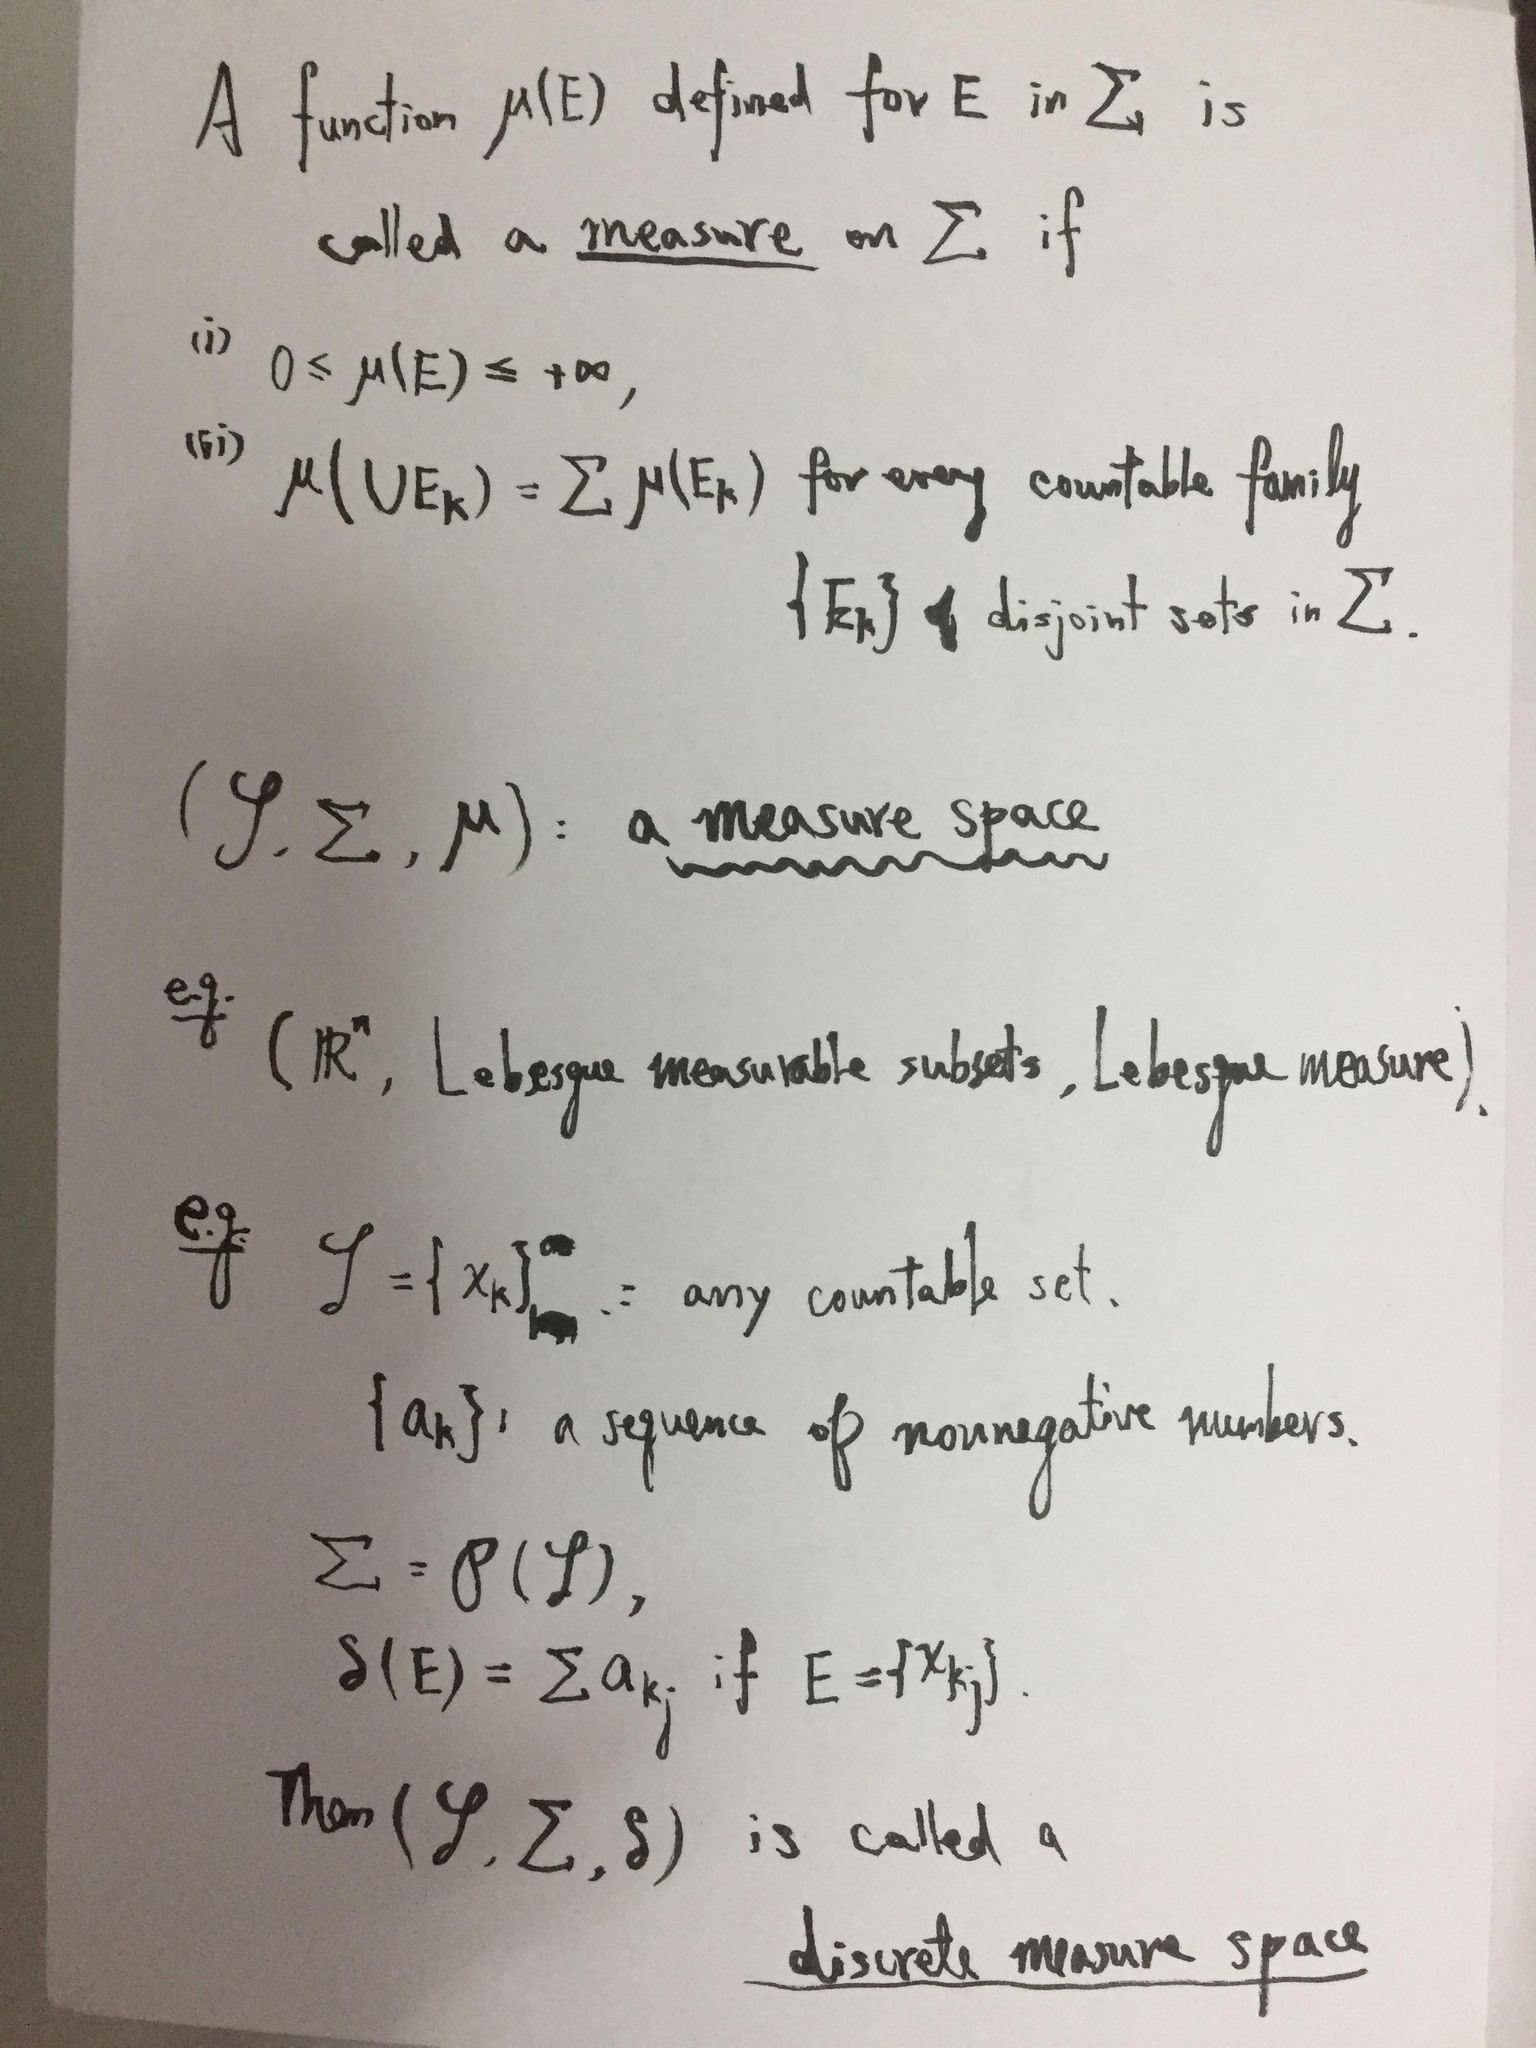
\includegraphics[scale=0.1]{measure_2.jpg} \medskip
\newpage
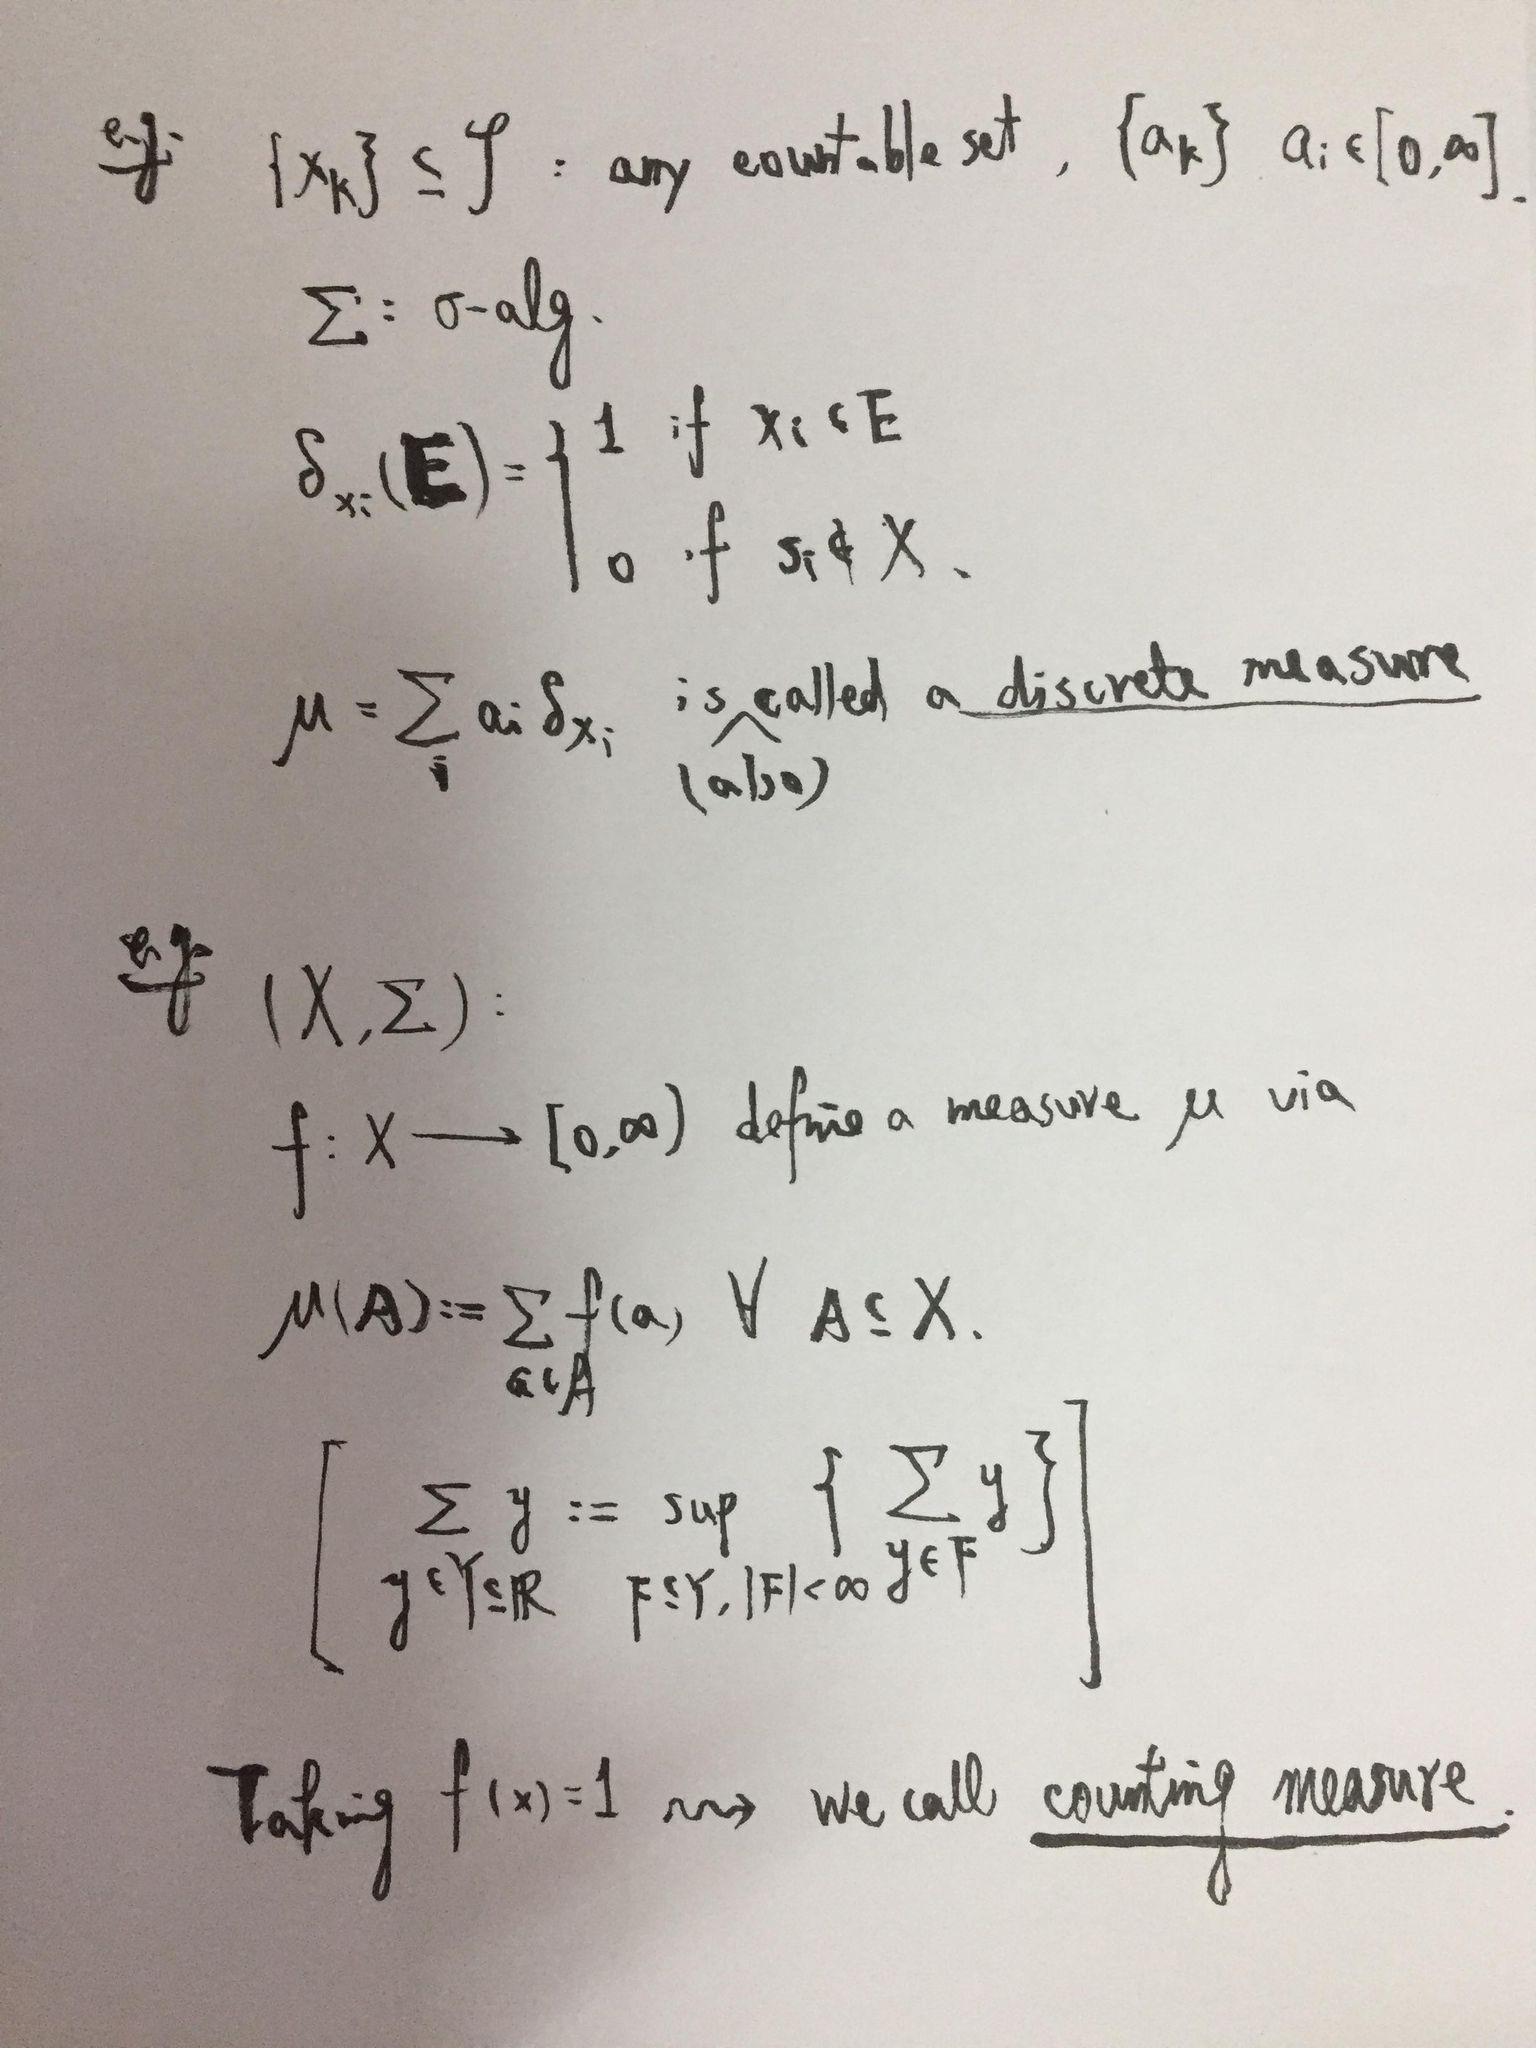
\includegraphics[scale=0.2]{measure_3.jpg}

\chapter{Distribution}

What is distribution ? \medskip

Let $\Omega$ be an open subset of $\mathbb{R}^n.$ The class of \textbf{test functions} $\mathcal{D}(\Omega)$ consists of all function $\phi(x)$ defined in $\Omega,$ vanishing outside a bounded subset of $\Omega$ that stays away from the boundary of $\Omega$ and $\phi \in C^\infty.$ \medskip

The class of distributions on $\Omega$ is defined to be all continuous linear functionals on $\mathcal{D}(\Omega).$\medskip

\section{Examples of distributions}
\begin{eg}[Dirac $\delta$ function]
$$
\langle \delta, \phi \rangle:=\phi(0).
$$

$$
\langle \delta^\prime, \phi \rangle:=-\phi^\prime(0).
$$
\end{eg}

\section{Operations on distributions} A operation $T$ on distributions means that $T\phi$ is a distribution for any distribution $\phi$ and $T$ is linear.

\begin{thm}
    Given any distribution $f \in \mathcal{D}^\prime (\Omega),$ there exists a sequence $\{\phi_n\}$ of test functions such that $\phi_n\rightarrow f$ as distributions.
\end{thm}

\chapter{Topology}
\section{Connected and Path-connected}
\begin{defi}
A topological space $X$ is called \textbf{connected} if any continuous map from $X$ to a discrete topological space is constant.
\end{defi}

\begin{prop}
A continuous map sends connected set to connected set. 
\end{prop}
\begin{proof}
From definition.
\end{proof}

\begin{prop}
Let $\{E_\alpha\}_{\alpha\in A}$ be a collection of connected spaces of a topological space $X.$ If any of two elements in $\{E_\alpha\}_{\alpha\in A}$ has nonempty intersection, then the union of $E_\alpha$ is connected. 
\end{prop}
\begin{proof}
Let $Y$ be their union. Then for any continuous map $f: Y\rightarrow D$ for some discrete topological space $D,$ we have $f|_{E_\alpha}$ is continuous, hence constant. Since any of two elements in $\{E_\alpha\}_{\alpha\in A}$ has nonempty intersection, $f$ must be constant. Therefore $Y$ is connected.
\end{proof}

\begin{prop}
Let $E$ be a connected set in a topological space $X.$ If $E\subset A \subset \overline{E}$, then $A$ is also connected. 
\end{prop}
\begin{proof}
For any continuous map $f: A\rightarrow D$ for some discrete topological space $D,$ then $f|_E$ is constant. Suppose $f|_A$ is not constant, i.e. there exist $a\in A, x\in E$ such that $f(a)$ is not $f(x).$ Then $f^{-1}(f(a))$ is an open neighborhood of $a$ and not intersects $E.$ This is a contradiction since $a\in \overline{E}.$ Thus $f|_A$ is constant. Hence, $A$ is connected.
\end{proof}

\begin{defi}
A topological space $X$ is called \textbf{path-connected} if for any $x,y\in X$ there is a continuous map $\gamma:[0,1]\rightarrow X$ such that $f(0)=x$ and $f(1)=y.$
\end{defi}

\begin{prop}
If a topological space $X$ is \textbf{path-connected}, then it is connected.
\end{prop}
\begin{proof}
First note that $[0,1]$ is connected and $\gamma$ is continuous; hence, $\gamma([0,1])$ is connected. For any continuous map $f: X\rightarrow D$ for some discrete topological space $D,$ we have $f|_{\gamma([0,1])}$ is constant. Since $X$ is path-connected we know that $f$ must be constant. 
\end{proof}

\begin{remark}
Path-connected and connected are kind of dual idea. Since \textbf{``path-connected''} consider the existence of maps into space $X$, and \textbf{``connected''} consider maps from $X$ to discrete spaces. (\textbf{``disconnected''} consider the existence of non-constant maps from $X$ to discrete spaces.)\medskip

Or we can define connected space $X$ to be ``For any $x,y\in X$ and any continuous map $f: X\rightarrow [0,1]$ with $f(x)=0, f(y)=1,$ we have $f(X)=[0,1].$'' This is \textbf{Intermediate Value Theorem.} So we can say in some sense that connected spaces are those spaces satisfy IVT. 
\end{remark}

\begin{prop}
Let $X$ be a topological space and $D$ be a connected topological space. Then any continuous map $f: D \rightarrow X$ sends $D$ into one of the connected components of $X.$
\end{prop}

\begin{cor}
For any subspace $D\subset X$, there is no continuous path $\gamma : [0,1] \rightarrow X$ with $f(0)\in int(D),$ $f(1)\in X\backslash \Bar{D}$ and $f(a)\not\in \partial D$ for all $a.$  
\end{cor}
\begin{proof}
Consider $Y=int(D) \bigcup (X\backslash \Bar{D})$ and use the proposition above. 
\end{proof}

\chapter{Algebraic Topology}
\begin{q}
For a topological space $M,$ does the assign from $M$ to its universal cover $\widetilde{M}\rightarrow M$ is a functor?
\end{q} No. I think we need to deal with uniqueness problem. For example, the map $(0,1)\rightarrow S^1$ has many liftings.\medskip

Many invariants in algebraic topology are homotopy invariant. \medskip

hTop: $Obj:$ Topological space $Morphism :$ continuous maps up to "homotopy" equivalence.\medskip

We have a canonical functor $\pi$: Top$\rightarrow$ hTop. Every functor, such as $\pi_n, H_n,$ which is homotopy functor is factor by functor $\pi:$ Top$\rightarrow$ hTop $\rightarrow$ homotopy functor. \medskip

\newpage
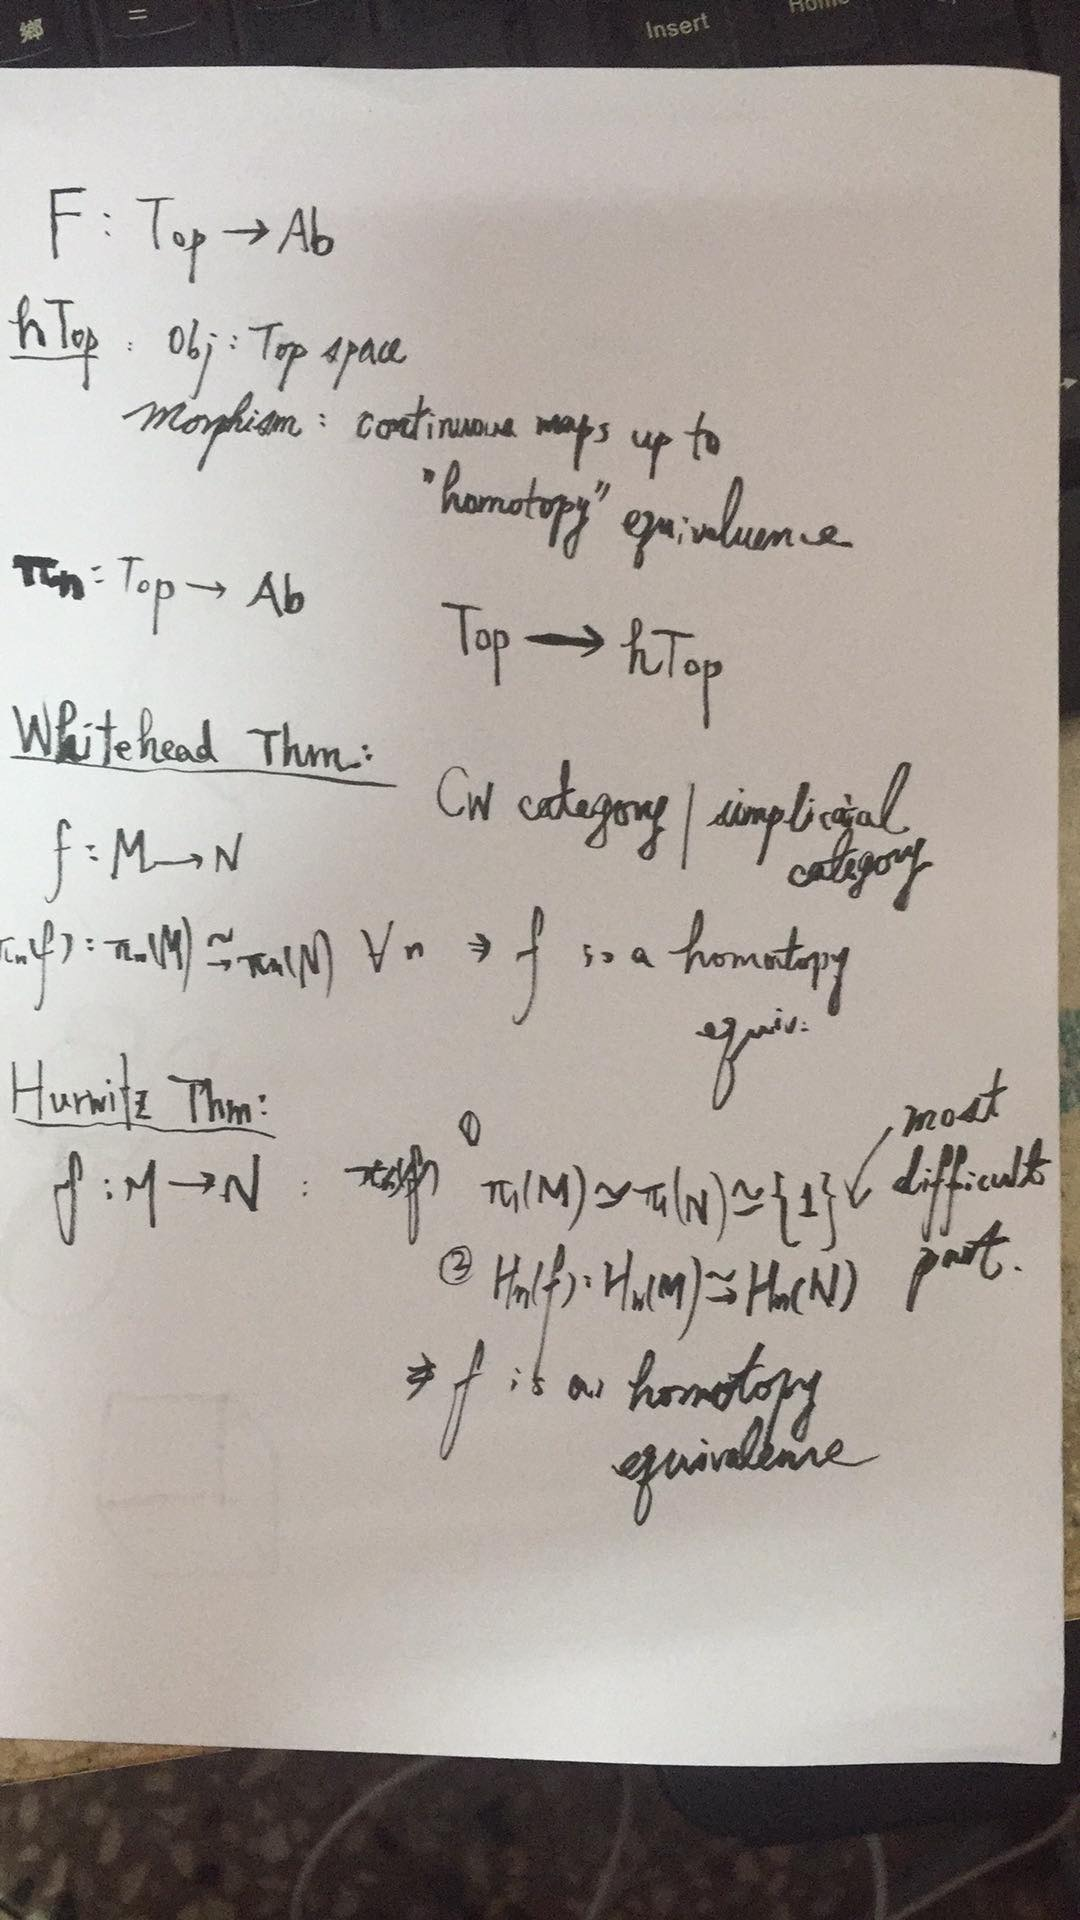
\includegraphics[scale=0.2]{homotopy.jpg}

\chapter{Counterexamples}
\begin{counter}
Let $E\subset \mathbb{R}^2$ be a non-empty open set and $f: E \rightarrow\mathbb{R}^2$
satisfy $f_x(x, y)=0$ on $E$, then $f(x, y)$ is a function of $y$ on $E$.
\end{counter}
\begin{proof}[(sol.)]
We have counterexamples for disconnected $E$ easily.\medskip

For connected $E$, I think the following example is a counterexample.\medskip

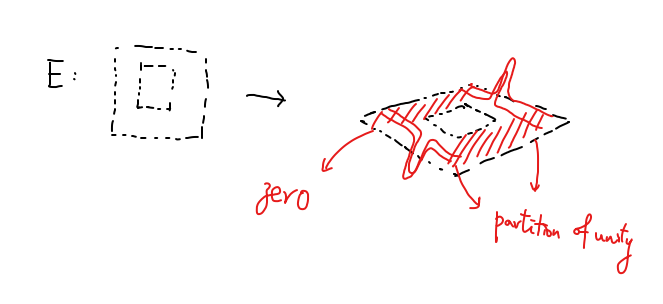
\includegraphics[scale=0.6]{partition of unity.PNG} \medskip
\end{proof}

\begin{counter}
For a locally compact space, a closed ball need not to be compact!
\end{counter}
\begin{proof}[(sol.)]
For example, one can take $X=\mathbb{R}\backslash \{0\},$ and the closed ball $\overline{B(1,2)}.$
\end{proof}

\begin{counter}[2023/04/09]
    Let $f: (0,\infty) \rightarrow \mathbb{R}$ be a function. If $\int_0^\infty f(x) dx$ exists, it does not imply $\lim_{x\rightarrow \infty}f(x) =0.$ 
\end{counter}
\begin{proof}[(sol.)]
Consider the functions has spike $1$ on integers $n$ with smaller width when $n$ goes to infinity. \medskip

Or one considers
$$
\int_0^\infty \sin(x^n) dx, n>1.
$$
\end{proof}

\chapter{Fact}
\begin{thm}
A bounded sequence having one limit point is convergent.
\end{thm}
\begin{proof}
Suppose $x_n\in R$ is bounded and has exactly one limit point. Then $x_n$ converges.\medskip

Suppose $x_{n_k}\to x$, and suppose $|x_n|\leq B$. \medskip

Let $\epsilon >0$, then $C_\epsilon=[-B,x-\epsilon]\cup[x+\epsilon,B]$ is a compact set, hence at most a finite number of $x_n\in C_\epsilon$ (otherwise there would be another limit point).

In particular, for all $\epsilon>0$ there is some $N$ such that for $n\geq N$, we have $|x-x_n|<\epsilon$. 
\end{proof}

\begin{thebibliography}{99}
\bibitem[N]{N} 
BAK, Joseph; NEWMAN, Donald J.; NEWMAN, Donald J. 
\textit{Complex analysis.} 
New York: Springer, 2010.

\bibitem[H]{H}
G. H. Hardy. 
\textit{Ramanujan. Twelve Lectures on subjects suggested by his life and work.}
Chelsea Publishing Company, New York, N.Y., 3rd edition, 1978.


\bibitem[S]{S} 
STEWART, James; CLEGG, Daniel K.; WATSON, Saleem.
\textit{Calculus:  early transcendentals.} 
Cengage Learning, 2020.

\bibitem[W]{W}
WHITTAKER,  Edmund  Taylor;  WATSON,  George  Neville.
\textit{A course of modern analysis.}
Cambridge university press, 1996.


\end{thebibliography}
\end{document}
